%!TEX TS-program = xelatex
\documentclass{beamer}

\usepackage{HSE-theme/beamerthemeHSE-en} % Load HSE theme

%%% Fonts 
\usepackage{fontspec}
%\defaultfontfeatures{Ligatures={TeX},Renderer=Basic}
%\setmainfont[Ligatures={TeX,Historic}]{Myriad Pro} % install Myriad Pro or replace with Arial
%\setsansfont{Myriad Pro}  % install Myriad Pro or replace with Arial
%\setmonofont{Courier New}

\usepackage{multicol} 		% Multiple columns
\graphicspath{{Images/}}  	% Images folder

 


%%% Author and speech
\title[Short title]{Globule-coil Transition in Models of Linear Magnetic Polymers} 
%\subtitle{Presentation Subtitle or Conference Title}
\author[Author's name]{Kamilla Faizullina \\ \smallskip \scriptsize \url{knfayzullina@edu.hse.ru}\\\url{  }}
\institute[Higher School of Economics]{National Research University \\ Higher School of Economics (Moscow)}
\date{\today}

\begin{document}	% Document begins

\frame[plain]{\titlepage}	% Title frame

\section{Just some text}
\subsection{Subtitle}

\begin{frame}
\frametitle{XY model on self-avoiding walks (SAWs)}
 	\begin{multicols}{2}
  
 		\begin{itemize}
 			\item Magnetic polymer is a sequence of $N$ monomers 
 			\item Conformation is a self-avoiding walk
 			\item Each node represents a spin-like variable $s_i$ associated with angle $\theta_i \in  [-\pi;\pi]$
 		\end{itemize}
   
 	\columnbreak
  
   \begin{figure}[H]
  	\centering
  	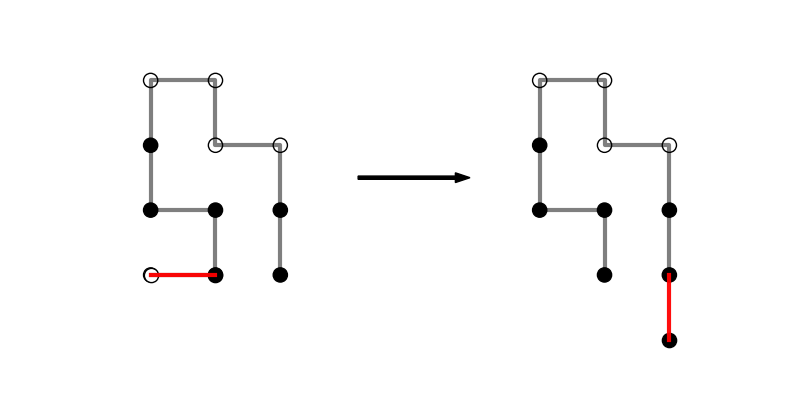
\includegraphics[scale=0.3]{snakeupdate.png}
  	%\caption{   }
  	\label{fig:example}
  \end{figure}
  
 \end{multicols}
\end{frame}



\begin{frame}
	\frametitle{XY model on self-avoiding walks (SAWs)}
	\begin{multicols}{2}
		
		\begin{itemize}
			\item Hamiltonian in lack of an external field: 
			\begin{equation*}
			H(u,s) = -J \sum_{ \langle i, j \rangle } cos(\theta_i - \theta_j)  
			\end{equation*}
			\item Partition function:
			
			
		\end{itemize}
		
		\columnbreak
		
		\begin{figure}[H]
			\centering
			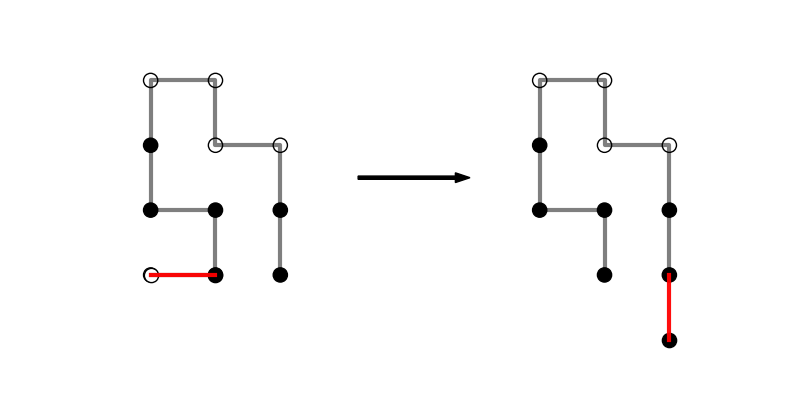
\includegraphics[scale=0.3]{snakeupdate.png}
			%\caption{   }
			\label{fig:example}
		\end{figure}
		
	\end{multicols}
\end{frame}



  

\end{document}